\documentclass[12pt]{article}
\setlength{\oddsidemargin}{12pt}
\setlength{\textwidth}{6.5in}
\setlength{\textheight}{9in}
\pagestyle{empty}
\setlength{\parskip}{7pt plus 2pt minus 2pt}
\usepackage{graphicx}
\graphicspath{ {images/} }

\begin{document}

\begin{center}
{{\large CS 330 : Discrete Computational Structures}}\\

{\bf Fall Semester, 2015}\\

{\sc Assignment \#4}\\
{\bf Due Date:}  Sunday, Sept 27\\

Cahlen Brancheau

\end{center}

\noindent {\bf Suggested Reading:} Rosen Sections 2.2 - 2.3; Lehman et al. Chapter 4.1, 4.3, 4.4

These are the problems that you need to turn in. For more
practice, you are encouraged to work on the other problems. Always
explain your answers and show your reasoning.

\begin{enumerate}

\item {\bf [4 Pts]} Use Venn Diagrams to prove that $(A - B) \cup (C - B) = (A \cup C) - B$.\\
\textbf{ANSWER:}\\
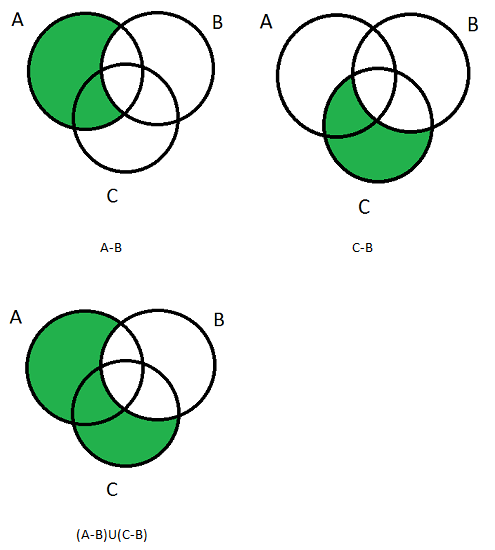
\includegraphics{Left}\\
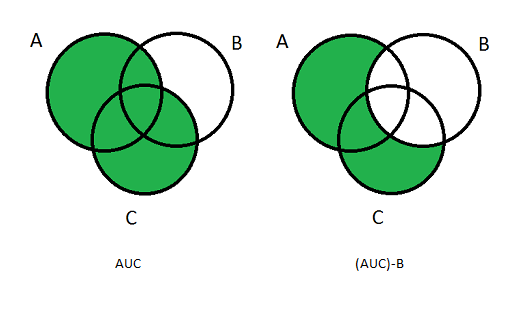
\includegraphics{Right}

\item {\bf [4 Pts]} Use an iff argument to prove that $(A - B) \cup (C - B) = (A \cup C) - B$. You may use logical equivalences in your proof.\\
\textbf{ANSWER:}\\
\begin{table}[h]
\centering
\begin{tabular}{ccll}
$x \in (A \cup C)-B$ & $\leftrightarrow$ & $x \in (A \cup C) \cap \overline{B}$                         & Def of Subtraction  \\
                  	       & $\leftrightarrow$ & $x \in (A \cup C) \wedge \overline{B}$                       & Def of $\cap$         \\
                		       & $\leftrightarrow$ & $x \in (A \cup C) \wedge \neg B$                             & Def of Compliment   \\
            	               & $\leftrightarrow$ & $x \in (A \vee C) \wedge \neg B$                             & Def of $\cup$         \\
                  	       & $\leftrightarrow$ & $x \in (A \wedge \neg B) \vee (C \wedge \neg B)$             & Def of Distributive \\
             	               & $\leftrightarrow$ & $x \in (A \wedge \neg B) \cup (C \wedge \neg B)$             & Def of $\cup$         \\
            	               & $\leftrightarrow$ & $x \in (A \wedge \overline{B}) \cup (C \wedge \overline{B})$ & Def of Compliment   \\
            	               & $\leftrightarrow$ & $x \in (A \cap \overline{B}) \cup (C \cap \overline{B})$ & Def of $\cap$   \\
                 	      & $\leftrightarrow$ & $x \in (A - B) \cup (C - B)$                                 & Def of Subtraction
\end{tabular}
\end{table}
\item {\bf [4 Pts]} Prove by contradiction that $(A - C) \cap (C - B) = \emptyset$.\\
\textbf{ANSWER:}\\

Suppose $(A - C) \cap (C - B) \neq \O$. So $x \in (A-C) \cap (C-B)$. 
Which means $x \in A$ and $x \notin C$ also $x \in C$ and $x \notin B$, contradiction. 
$x$ cannot both be in and not in $C$. 
Therefore $(A-C) \cap (C-B) = \O$.

\clearpage
\item {\bf [6 Pts]} Disprove the statements below.
\begin{enumerate}
\item If $A \cup C = B \cup C$ then $A= B$.\\\\
\textbf{ANSWER:}\\
$A = \{ 1,2,3 \}$\\
$B = \{ 1,2,3,4 \}$\\
$C = \{ 1,2,3,4 \}$\\\\
$A \cup C = \{ 1,2,3,4 \}$\\
$B \cup C = \{ 1,2,3,4 \}$\\
$A \neq B$\\
\item If $A \cap C = B \cap C$ then $A= B$.\\\\
\textbf{ANSWER:}\\
$A = \{ a,b,c \}$\\
$B = \{ a,b \}$\\
$C = \{ a,b \}$\\\\
$A \cap C = \{ a,b \}$\\
$B \cap C = \{ a,b \}$\\
$A \neq B$\\

\end{enumerate}

\item {\bf [6 Pts]} Prove that if $A \cup C = B \cup C$ and $A \cap C = B \cap C$ then $A= B$.\\\\
\textbf{ANSWER:}\\
If $A = \{ a,b \}$, $B = \{ a,b \}$,  $C = \{ b,c \}$\\
Then $A \cup C = \{ a,b,c \}$ and $B \cup C = \{ a,b,c \}$\\
Then $A \cap C = \{ b \}$ and $B \cup C = \{ b \}$\\
Therefore $A=B$\\

\clearpage
\item {\bf [8 Pts]} Prove by subset argument (in both directions) that $\overline{A \cup B} = \overline{A} \cap \overline{B}$. 
         You {\it may not} use logical equivalences in your proof. \\\\
	\textbf{ANSWER:}\\
         (1) $\overline{A \cup B} \subseteq \overline{A} \cap \overline{B}$\\
         (2) $ \overline{A} \cap \overline{B}  \subseteq \overline{A \cup B}  $\\\\
         
         (1) Let $x \in \overline{A \cup B}$. We prove $x \in \overline{A} \cap \overline{B}$.\\
         So we have $x \notin A \cup B$ by the definition of complement.\\
         	(a) Suppose $x \in A$ then $x \in A \cup B$, contradiction. So $x \in \overline{A}$.\\
	
		(b) Suppose $x \in B$ then $x \in A \cup B$, contradiction. So $x \in \overline{B}$.\\
	By definition of $\cap$ we have $\overline{A} \cap \overline{B}$.\\
	Therefore $\overline{A \cup B} \subseteq \overline{A} \cap \overline{B}$\\\\
				
	(2) Let $x \in \overline{A} \cap \overline{B}$. We prove $x \in \overline{A \cup B}$.\\
	So we have $x \in \overline{A}$ and $x \in \overline{B}$ by the definition of $\cap$\\
	and we have $x \notin A$ and $x \notin B$ by the definition of complement\\
	Suppose $x \notin \overline{A \cup B}$ then by definition of complement we have $x \in A \cup B$\\
		(a) $x \in A$, contradiction. $x \notin A$\\
		(B) $x \in B$, contradiction. $x \notin B$\\ 
	Therefore $\overline{A \cup B}$.\\
	
				
\clearpage
\item {\bf [4 Pts]} Consider the function $f$ mapping $\cal R$ to $\cal R$, where $f(n) = 3n^2 - 8$.

\begin{enumerate}
\item Explain why $f$ is neither one-to-one nor onto. \\
	\textbf{ANSWER:}\\
	$f(1) = 3(1)^2 - 8 = -5$\\
	$f(-1) = 3(-1)^2 - 8 = -5$\\
	but $1 \neq -1$ therefor f is not One-To-One\\
	
\item Now, restrict either the domain or co-domain to make $f$ one-to-one. \\
	\textbf{ANSWER:}\\
	Restricting the domain to map from $\cal R^+$ to $\cal R$ removes negative numbers making f One-To-One.  \\

\item Then, restrict either the domain or co-domain to make $f$ onto.\\
	\textbf{ANSWER:}\\
	Restricting the co-domain to map from $\cal R^+$ to $\cal R^+$ removes negative numbers that cannot be mapped from the domain making f Onto.  \\
	
\end{enumerate}

\item {\bf [4 Pts]} Prove that $f(n) = 3n + 5$ is one-to-one,  where the domain and co-domain of $f$ is $\cal Z^+$. Show that $f$ is not onto.\\
	\textbf{ANSWER:}
\begin{table}[h]
\centering
\begin{tabular}{ccc}
$3x + 5$ & $=$ & $3y + 5$ \\
$3x$     & $=$ & $3y$     \\
$x$      & $=$ & $3y + 5$
\end{tabular}
\end{table}\\
Therefore f is One-To-One\\
\begin{table}[h]
\centering
\begin{tabular}{ccc}
$3x + 5$ & $=$ & $1$            \\
$3x$     & $=$ & $-4$           \\
$x$      & $=$ & $\frac{-4}{3}$
\end{tabular}
\end{table}\\
$1 \in \cal Z^+$ therefore in the co-domain, but $\frac{-4}{3} \notin \cal Z^+$ therefore  not in the domain. So there does not exist an $x$ that maps to $1$. So f is not Onto.
	
\clearpage
\item {\bf [4 Pts]} Prove that $f(m,n) = m + n - 2$ is onto,  where the domain of $f$ is ${\cal Z} \times {\cal Z}$ and the co-domain of $f$ is $\cal Z$. Show that $f$ is not one-to-one. \\
	\textbf{ANSWER:}\\
	$f(2,-2) = f(-2,2) = -2$ but $(2,-2) \neq (-2,2)$ therefore f is not Ont-To-One\\\\
	
	Let $t = m+n-2$. Find $m,n \in \cal Z$ S.T. $m+n - 2 = t$\\
	$x=t$, $y=2$\\
	$x=2$, $y=t$\\
	Therefore f is Onto
				
\item {\bf [6 Pts]} Prove that $f(m,n) = (m+n, m-n)$ is one-to-one and onto,  where the domain and co-domain of $f$ is ${\cal R} \times {\cal R}$.
         Give the inverse function of $f$.

\end{enumerate}
\end{document}


